\let\negmedspace\undefined
\let\negthickspace\undefined
\documentclass[journal]{IEEEtran}
\usepackage[a5paper, margin=10mm, onecolumn]{geometry}
%\usepackage{lmodern} % Ensure lmodern is loaded for pdflatex
\usepackage{tfrupee} % Include tfrupee package

\setlength{\headheight}{1cm} % Set the height of the header box
\setlength{\headsep}{0mm}     % Set the distance between the header box and the top of the text
\usepackage{xparse}
\usepackage{gvv-book}
\usepackage{gvv}
\usepackage{cite}
\usepackage{amsmath,amssymb,amsfonts,amsthm}
\usepackage{algorithmic}
\usepackage{graphicx}
\usepackage{textcomp}
\usepackage{xcolor}
\usepackage{txfonts}
\usepackage{listings}
\usepackage{enumitem}
\usepackage{mathtools}
\usepackage{gensymb}
\usepackage{comment}
\usepackage[breaklinks=true]{hyperref}
\usepackage{tkz-euclide} 
\usepackage{listings}
% \usepackage{gvv}                                        
\def\inputGnumericTable{} 
\usepackage[latin1]{inputenc}                                
\usepackage{color}                                            
\usepackage{array}                                            
\usepackage{longtable}                                       
\usepackage{calc}                                             
\usepackage{multirow}                                         
\usepackage{hhline}                                           
\usepackage{ifthen}                                           
\usepackage{lscape}

\begin{document}

\bibliographystyle{IEEEtran}
\vspace{3cm}

\title{GATE Questions 21}
\author{EE24BTECH11012 - Bhavanisankar G S}
% \maketitle
% \newpage
% \bigskip
{\let\newpage\relax\maketitle}
\begin{enumerate}
	\item You should \rule{1cm}{0.1pt} when to say \rule{1cm}{0.1pt}.
		\begin{enumerate}
				\begin{multicols}{2}
				\item no, no
				\item no, know
				\item know, know
				\item know, no
				\end{multicols}
		\end{enumerate}
	\item Two straight lines pass though the origin $\brak{x_0, y_0} = \brak{0,0}$. One of them passes through the point $\brak{x_1, y_1} = \brak{1,3}$ and the other passes through the point $\brak{x_2, y_2} = \brak{1,2}$. \\
		What is the area enclosed between the straight lines in the interval \sbrak{0,1} on the $x$-axis ?
		\begin{enumerate}
				\begin{multicols}{4}
				\item 0.5
				\item 1.0
				\item 1.5
				\item 2.0
				\end{multicols}
		\end{enumerate}
	\item If 
				$$ p : q = 1 : 2 $$
				$$ q : r = 4 : 3 $$
				$$ r : s = 4 : 5 $$
				and $u$ is 50 \% more than $s$, then what is the ratio of $p:u$ ?
				\begin{enumerate}
						\begin{multicols}{4}
						\item 2:15
						\item 16:15
						\item 1:5
						\item 16:45
						\end{multicols}
				\end{enumerate}
	\item Given the statements : \\
		P is the sister of Q \\
		Q is the husband of R \\
		R is the mother of S \\
		T is the husband of P \\
		Based on the above information, T is \rule{1cm}{0.1pt} of S.
		\begin{enumerate}
				\begin{multicols}{4}
				\item the grandfather
				\item an uncle
				\item the father
				\item a brother
				\end{multicols}
		\end{enumerate}
	\item In the following diagram, the point R is the centre of the circle. The lines PQ and ZV are tangential to the circle. The relation among the areas of the squares, PXWR, RUVZ and SPQT is
		\begin{figure}[H]
			\centering
			\begin{circuitikz}
\tikzstyle{every node}=[font=\normalsize]
\draw  (5.5,7.75) circle (2.5cm);
\draw  (7.75,9.875) -- (5.375,12.375) -- (3,9.875) -- (5.375,7.375) -- cycle;
\draw [short] (3,7.5) -- (7.5,7.5);
\draw [short] (7,7.5) -- (8,7.5);
\draw [short] (5.5,7.5) -- (5.5,5.25);
\draw [short] (8,7.5) -- (8,5.25);
\draw [short] (5.5,5.25) -- (8,5.25);
\draw [short] (3,7.5) -- (3,10);
\draw [short] (3,7.5) -- (1,7.5);
\draw [short] (1,7.5) -- (1,10);
\draw [short] (1,10) -- (3,10);
\node [font=\normalsize] at (2.75,10.25) {P};
\node [font=\normalsize] at (1,10.5) {S};
\node [font=\normalsize] at (0.75,7.5) {T};
\node [font=\normalsize] at (2.75,7.75) {Q};
\node [font=\normalsize] at (5.5,7.75) {R};
\node [font=\normalsize] at (5.5,12.75) {X};
\node [font=\normalsize] at (5.25,5.5) {U};
\node [font=\normalsize] at (8.25,10) {W};
\node [font=\normalsize] at (8.25,7.75) {Z};
\node [font=\normalsize] at (8.5,5.25) {V};
\end{circuitikz}

			\label{tab: Q_5}
		\end{figure}
		\begin{enumerate}
			\item Ar(SPQT) = Ar(RUVZ) + Ar(PXWR)
			\item Ar(SPQT) = Ar(PXWR) + Ar(RUVZ)
			\item Ar(PXWR) = Ar(SPQT) - Ar(RUVZ)
			\item Ar(PXWR) = Ar(RUVZ) - Ar(SPQT)
		\end{enumerate}
	\item Healthy eating is a critical component of healthy ageing. When should one start eating healthy ? It turns out that it is never too early. For example, babies who start eating healthy in the first year are more likely to have better overall health as they get older. \\
		Which one of the following is the CORRECT logical inference based on the information in the above passage ?
		\begin{enumerate}
			\item Healthy eating is important for those with good health conditions, but not for others.
			\item Eating healthy can be started at any age, earlier the better.
			\item Eating healthy and better overall health are more correlated at a young age, but not older age.
			\item Healthy eating is more important for adults than kids.
		\end{enumerate}
	\item P invested rupees 5000 per month for 6 months of a year and Q invested rupess $x$ per month for 8 months of the year in a partnership business. The profit is shared in proportion to the total investment in that year. \\
		If at the end of that investment year, Q receives $\frac{4}{9}$ of the total profit, what is the value of $x$ ( in rupees ) ?
		\begin{enumerate}
				\begin{multicols}{4}
				\item 2500
				\item 3000
				\item 4687
				\item 8437
				\end{multicols}
		\end{enumerate}
	\item The frequency chart below shows the frequency distribution of marks obtained by a set of students in an exam . \\
		\begin{figure}[H]
			\centering
			\begin{tikzpicture}
\draw[->] (0,0) -- (8,0) node[right] {Marks} ;
\draw[->] (0,0) -- (0,8) node[above] {Frequency} ;

\draw[fill=black] (0.5,0) rectangle (1,1.5) ;
\draw[fill=black] (1.5,0) rectangle (2,4.5) ;
\draw[fill=black] (2.5,0) rectangle (3,5.5) ;
\draw[fill=black] (3.5,0) rectangle (4,3.5) ;
\draw[fill=black] (4.5,0) rectangle (5,7) ;
\draw[fill=black] (5.5,0) rectangle (6,1) ;
\draw[fill=black] (6.5,0) rectangle (7,2) ;

\node at (0.5,0) {3} ;
\node at (1.5,0) {4} ;
\node at (2.5,0) {5} ;
\node at (3.5,0) {6} ;
\node at (4.5,0) {7} ;
\node at (5.5,0) {8} ;
\node at (6.5,0) {9} ;

\node at (0,1) {2} ;
\node at (0,2) {4} ;
\node at (0,3) {6} ;
\node at (0,4) {8} ;
\node at (0,5) {10} ;
\node at (0,6) {12} ;
\node at (0,7) {14} ;
\node at (0,8) {16} ;

\end{tikzpicture}

			\label{tab: Q_8}
		\end{figure}
		From the data presented above, which of the following is CORRECT ?
		\begin{enumerate}
			\item mean $>$ mode $>$ median
			\item mode $>$ median $>$ median
			\item mode $>$ mean $>$ median
			\item median $>$ mode $>$ mean
		\end{enumerate}
	\item In the suare grid shown below, a person standing at P2 position is required to move to p5 position. \\
		\begin{figure}[H]
			\centering
			\begin{tikzpicture}
\draw[->] (0,0) -- (5,0) ;
\draw[->] (0,0) -- (0,5) ;

\draw[fill=white] (0,0) rectangle (1,1) ;
\draw[fill=white] (1,0) rectangle (2,1) ;
\draw[fill=black] (2,0) rectangle (3,1) ;
\draw[fill=white] (3,0) rectangle (4,1) ;
\draw[fill=white] (4,0) rectangle (5,1) ;
\draw[fill=white] (0,1) rectangle (1,2) ;
\draw[fill=black] (1,1) rectangle (2,2) ;
\draw[fill=white] (2,1) rectangle (3,2) ;
\draw[fill=white] (3,1) rectangle (4,2) ;
\draw[fill=black] (4,1) rectangle (5,2) ;
\draw[fill=black] (0,2) rectangle (1,3) ;
\draw[fill=white] (1,2) rectangle (2,3) ;
\draw[fill=white] (2,2) rectangle (3,3) ;
\draw[fill=white] (3,2) rectangle (4,3) ;
\draw[fill=white] (4,2) rectangle (5,3) ;
\draw[fill=white] (0,3) rectangle (1,4) ;
\draw[fill=white] (1,3) rectangle (2,4) ;
\draw[fill=black] (2,3) rectangle (3,4) ;
\draw[fill=white] (3,3) rectangle (4,4) ;
\draw[fill=white] (4,3) rectangle (5,4) ;
\draw[fill=black] (0,4) rectangle (1,5) ;
\draw[fill=white] (1,4) rectangle (2,5) ;
\draw[fill=white] (2,4) rectangle (3,5) ;
\draw[fill=black] (3,4) rectangle (4,5) ;
\draw[fill=white] (4,4) rectangle (5,5) ;

\node at (0,5,5.5) {1} ;
\node at (1.5,5.5) {2} ;
\node at (2.5,5.5) {3} ;
\node at (3.5,5.5) {4} ;
\node at (4.5,5.5) {5} ;

\node at (-0.5,0.5) {T} ;
\node at (-0.5,1.5) {S} ;
\node at (-0.5,2.5) {R} ;
\node at (-0.5,3.5) {Q} ;
\node at (-0.5,4.5) {P} ;

\end{tikzpicture}


			\label{tab: Q_9}
		\end{figure}
		The only movement allowed for a step involves, " two moves along one direction followed by one move in a perpendicular direction ". %The permissible directions for movement are shown as dotted arrows in the right. \\
		%For example, a person at a given position \textbf{Y} can move only to the position marked \textbf{X} on the right. \\
		Without occupying any of the shaded squares at the end of each step, the minimum number of steps required to go from P2 to P5 is
		\begin{enumerate}
				\begin{multicols}{4}
				\item 4
				\item 5
				\item 6
				\item 7
				\end{multicols}
		\end{enumerate}
	\item Consider a cube made by folding a single sheet of paper of appropriate shape. The interior faces of the cube are all blank. However, the exterior faces that are not visible in the above view may not be blank. \\
		Which one of the following represents a possible unfolding of the  cube ?
		\begin{multicols}{2}
			\begin{enumerate}
				\item
					\begin{figure}[H]
			\centering
			\begin{tikzpicture}

\draw[fill=white] (0,2) rectangle (1,3) ;
\draw[fill=white] (1,2) rectangle (2,3) ;
\draw[fill=white] (1,1) rectangle (2,2) ;
\draw[fill=gray] (1,0) rectangle (2,1) ;
\draw[fill=black] (2,1) rectangle (3,2) ;
\draw[fill=white] (3,1) rectangle (4,2) ;

\end{tikzpicture}

			\label{tab: Q_10a}
		\end{figure}
				\item
					\begin{figure}[H]
			\centering
			\input{figs/10b.tex}
			\label{tab: Q_10b}
		\end{figure}
				\item
					\begin{figure}[H]
			\centering
			\begin{tikzpicture}

\draw[fill=white] (0,0) rectangle (1,1) ;
\draw[fill=white] (1,0) rectangle (2,1) ;
\draw[fill=white] (3,0) rectangle (4,1) ;
\draw[fill=gray] (1,1) rectangle (2,2) ;
\draw[fill=black] (2,0) rectangle (3,1) ;
\draw[fill=white] (3,1) rectangle (4,2) ;

\end{tikzpicture}

			\label{tab: Q_10c}
		\end{figure}
				\item
					\begin{figure}[H]
			\centering
			\begin{tikzpicture}

\draw[fill=white] (3,1) rectangle (4,2) ;
\draw[fill=white] (2,1) rectangle (3,2) ;
\draw[fill=white] (1,1) rectangle (2,2) ;
\draw[fill=gray] (1,0) rectangle (2,1) ;
\draw[fill=black] (0,1) rectangle (1,2) ;
\draw[fill=white] (3,2) rectangle (4,3) ;

\end{tikzpicture}

			\label{tab: Q_10d}
		\end{figure}
			\end{enumerate}
		\end{multicols}
	\item For the Op-Amp circuit shown below, choose the correct output waveform corresponding to the input $V_{in} = 1.5 \sin{20 \pi t}$ ( in Volts ). The saturation voltage for this circuit is $V_{sat} = \pm 10 V$
		\begin{figure}[H]
			\centering
			\begin{circuitikz}
\tikzstyle{every node}=[font=\normalsize]
\draw (3.75,10.25) node[op amp,scale=1] (opamp2) {};
\draw (opamp2.+) to[short] (2.25,9.75);
\draw  (opamp2.-) to[short] (2.25,10.75);
\draw (4.95,10.25) to[short](5.25,10.25);
\draw (2.25,9.75) to[R] (2.25,6);
\draw (2.25,8.5) to[R] (6.75,8.5);
\draw (3.75,10.75) to[short] (3.75,12.25);
\draw (3.75,9.75) to[short] (3.75,9);
\draw (3.75,10) to[short] (3.75,9.25);
\draw (3.75,10.5) to[short] (3.75,11.5);
\draw (6.75,8.5) to[short] (6.75,10.25);
\draw (6.75,10.25) to[short] (5,10.25);
\draw (2.25,10.75) to[short] (0,10.75);
\draw (0,10.75) to[sinusoidal voltage source, sources/symbol/rotate=auto] (0,8.75);
\draw (2.25,6.5) to (2.25,6) node[ground]{};
\draw (0,9) to (0,7.75) node[ground]{};
\node [font=\normalsize] at (-0.5,9.25) {$V_{in}$};
\node [font=\normalsize] at (1.5,8) {2.2 k $\Omega$};
\node [font=\normalsize] at (4.25,8) {20 k$\Omega$};
\node [font=\normalsize] at (6,10.5) {$V_{out}$};
\end{circuitikz}

			\label{tab: Q_11}
		\end{figure}
		%\begin{multicols}{2}
			\begin{enumerate}
				\item
					\begin{figure}[H]
			\centering
			\begin{circuitikz}
\tikzstyle{every node}=[font=\normalsize]
\draw (1.25,6) to[short] (1.25,12.25);
\draw (1.25,6) to[short] (7.5,6);
\draw (1.25,11) to[short] (1.75,11);
\draw (1.75,11) to[short] (1.75,6.5);
\draw (1.75,6.5) to[short] (3,6.5);
\draw (3,6.5) to[short] (3,11);
\draw (3,11) to[short] (4.25,11);
\draw (4.25,11) to[short] (4.25,6.5);
\draw (4.25,6.5) to[short] (5.5,6.5);
\draw (5.5,6.5) to[short] (5.5,11);
\draw (5.5,11) to[short] (6.75,11);
\draw (6.75,11) to[short] (6.75,6.5);
\draw (6.75,6.5) to[short] (7.75,6.5);
\node [font=\normalsize] at (4,5.5) {Time};
\node [font=\normalsize, rotate around={90:(0,0)}] at (0.25,8.75) {$V_{out}$ ( volts )};
\node [font=\normalsize] at (1,6.5) {-10};
\node [font=\normalsize] at (1,7.5) {-5};
\node [font=\normalsize] at (1,8.5) {0};
\node [font=\normalsize] at (1,9.75) {5};
\node [font=\normalsize] at (1,11) {10};
\end{circuitikz}

			\label{tab: Q_11a}
		\end{figure}
				\item
					\begin{figure}[H]
			\centering
			\begin{circuitikz}
\tikzstyle{every node}=[font=\normalsize]
\draw (1.25,6) to[short] (1.25,12.25);
\draw (1.25,6) to[short] (7.5,6);
\node [font=\normalsize] at (4,5.5) {Time};
\node [font=\normalsize, rotate around={90:(0,0)}] at (0.25,8.75) {$V_{out}$ ( volts )};
\node [font=\normalsize] at (1,6.5) {-10};
\node [font=\normalsize] at (1,7.5) {-5};
\node [font=\normalsize] at (1,8.5) {0};
\node [font=\normalsize] at (1,9.75) {5};
\node [font=\normalsize] at (1,11) {10};
\draw (1.25,11) to[short] (7.5,11);
\end{circuitikz}

			\label{tab: Q_11b}
		\end{figure}
				\item
					\begin{figure}[H]
			\centering
			\begin{circuitikz}
\tikzstyle{every node}=[font=\normalsize]
\draw (1.25,6) to[short] (1.25,12.25);
\draw (1.25,6) to[short] (7.5,6);
\node [font=\normalsize] at (4,5.5) {Time};
\node [font=\normalsize, rotate around={90:(0,0)}] at (0.25,8.75) {$V_{out}$ ( volts )};
\node [font=\normalsize] at (1,6.5) {-10};
\node [font=\normalsize] at (1,7.5) {-5};
\node [font=\normalsize] at (1,8.5) {0};
\node [font=\normalsize] at (1,9.75) {5};
\node [font=\normalsize] at (1,11) {10};
\draw [short] (1.25,8.5) .. controls (2,14.25) and (3,8.25) .. (3,8.5);
\draw [short] (3,8.5) .. controls (3.75,4) and (4.5,8) .. (4.5,8.5);
\draw [short] (4.5,8.5) .. controls (5,14.25) and (5.75,8.25) .. (5.75,8.5);
\draw [short] (5.75,8.5) .. controls (6.5,3.5) and (7.75,9.25) .. (7.5,8.5);
\end{circuitikz}

			\label{tab: Q_11c}
		\end{figure}
				\item
					\begin{figure}[H]
			\centering
			\input{figs/11d.tex}
			\label{tab: Q_11d}
		\end{figure}
			\end{enumerate}
		%\end{multicols}
	\item Match the order of $\beta^{-1}$ decays given in the left column to appropriate clause in the right column. Here $X(i^{\pi}) \text{and} Y(I^{\pi})$ are nuclei with intrinsic spin $I$ and parity $\pi$.
		\begin{table}[H]
\centering
\begin{tabular}{|c|c|}
\hline
$X \brak{\frac{1}{2} ^{+}} \to Y \brak{\frac{1}{2} ^{+}}$ & (i) First forbidden $\beta$-decay \\
\hline
$X \brak{\frac{1}{2} ^{-}} \to Y \brak{\frac{5}{2} ^{+}}$ & (ii) Second forbidden $\beta$-decay \\
\hline
$X \brak{ 3^{+}} \to Y \brak{0^{+}}$ & (iii) Third forbidden $\beta$-decay \\
\hline
$X \brak{4^{-}} \to Y \brak{0^{+}}$ & (iv) Allowed $\beta$-decay \\
\hline
\end{tabular}
\label{tab: Q_12}
\end{table}

		\begin{enumerate}
				\begin{multicols}{2}
				\item 1 - i, 2 - ii, 3 - iii, 4 - iv
				\item 1 - iv, 2 - 1, 3 - ii, 4 - iii
				\item 1 - i, 2 - iii, 3 - ii, 4 - iv
				\item 1 - iv, 2 - ii, 3 - iii, 4 - i
				\end{multicols}
		\end{enumerate}
	\item What is the maximum number of free independent real parameters specifying an n-dimensional orthogonal matrix ?
		\begin{enumerate}
				\begin{multicols}{4}
				\item $n(n-2)$
				\item $\brak{n-1}^2$
				\item $\frac{n(n-1)}{2}$
				\item $\frac{n(n+1)}{2}$
				\end{multicols}
		\end{enumerate}
\end{enumerate}
\end{document}

